\documentclass{beamer}
\usetheme{Dresden}
%\usetheme{CambridgeUS}
\usepackage{helvet}
\usepackage{cite}
\usepackage{url}
\usepackage{amssymb, amsmath, graphicx, charter, latexsym}
\usepackage{subfigure}
\usepackage{enumerate}
\usepackage{ragged2e}
\usepackage{mathtools}
\usepackage{tabu}
\usepackage{epstopdf}
\usepackage{siunitx}
\renewcommand{\familydefault}{\sfdefault}
%\usepackage{times}
\setbeamertemplate{items}[circle]
\setbeamertemplate{navigation symbols}{}
\begin{document}
\title{S-WiFi: Scheduling for Uplink Transmissions with Point Coordination Function}
\author{Dongni Han, Ping-Chun Hsieh, and Tao Zhao}
\date{April 29, 2016}
\newtheorem{thm}{Theorem} 
\begin{frame}
\titlepage
\end{frame}


%\begin{frame}
%\frametitle{What to Discuss Today?}
%\tableofcontents[]
%\end{frame}

%\AtBeginSection[]
%{
	%\begin{frame}{Table of Contents}
	%\tableofcontents[currentsection]
	%\end{frame}
%}


\section{Baseline Review}

\begin{frame}
\frametitle{Uplink Transmissions}
\begin{itemize}
\item One AP and N clients
\item 1 slot = 10ms; 1 interval = $T$ slots
\item Packets generated in the beginning of each interval
\item Packet generation follows Unif$\{Rmin, Rmax\}$
\item Real-time traffic
\end{itemize}
\begin{figure}
\centering
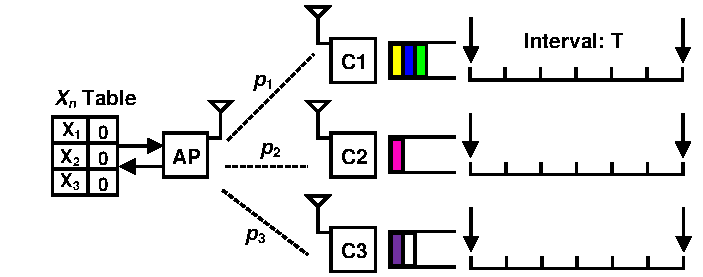
\includegraphics[scale=0.8]{network.pdf}
\end{figure}
\end{frame}

\begin{frame}
\frametitle{Baseline Policy - A Toy Example}
\begin{itemize}
\item $N=3$ and $T=6$
\item $p_1 = p_2 = p_3 = 0.5$
\item Real-time traffic
\item $X_n(k) =$ queue length at the start of the $k$-th interval 
\end{itemize}
\begin{figure}
\centering
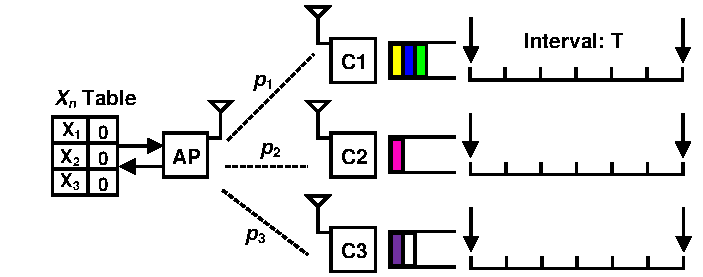
\includegraphics[scale=0.8]{network.pdf}
\end{figure}
\end{frame}

\begin{frame}
\frametitle{Baseline Policy - A Toy Example}
\begin{itemize}
\item Phase 1: AP polls $X_n$ in a round-robin manner
\end{itemize}
\begin{figure}
\centering
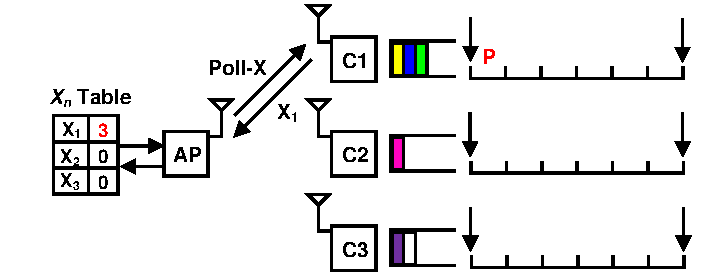
\includegraphics[scale=0.8]{animation_01.pdf}
\end{figure}
\end{frame}

\begin{frame}
\frametitle{Baseline Policy - A Toy Example}
\begin{itemize}
\item Phase 1: AP polls $X_n$ in a round-robin manner
\end{itemize}
\begin{figure}
\centering
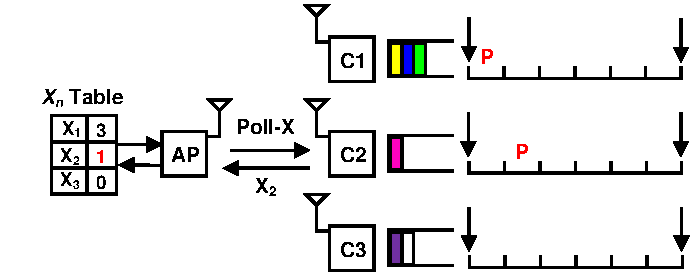
\includegraphics[scale=0.8]{animation_02.pdf}
\end{figure}
\end{frame}

\begin{frame}
\frametitle{Baseline Policy - A Toy Example}
\begin{itemize}
\item Phase 1: AP polls $X_n$ in a round-robin manner
\end{itemize}
\begin{figure}
\centering
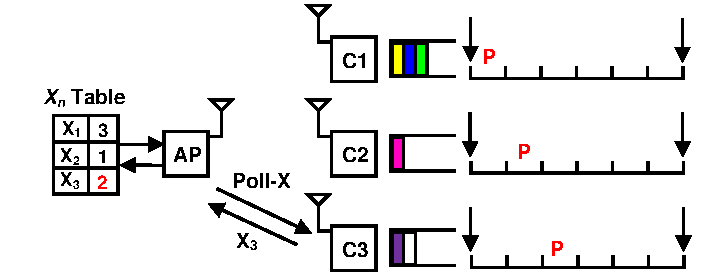
\includegraphics[scale=0.8]{animation_03.pdf}
\end{figure}
\end{frame}

\begin{frame}
\frametitle{Baseline Policy - A Toy Example}
\begin{itemize}
\item Phase 2: AP schedules a client based on Max-Weight policy
\item Max-Weight: select the client that maximizes $p_nX_n$
\end{itemize}
\begin{figure}
\centering
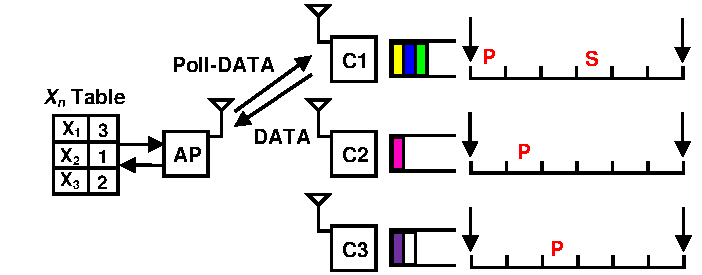
\includegraphics[scale=0.8]{animation_04.pdf}
\end{figure}
\end{frame}

\begin{frame}
\frametitle{Baseline Policy - A Toy Example}
\begin{itemize}
\item Phase 2: AP schedules a client based on Max-Weight policy
\item Max-Weight: select the client that maximizes $p_nX_n$
\end{itemize}
\begin{figure}
\centering
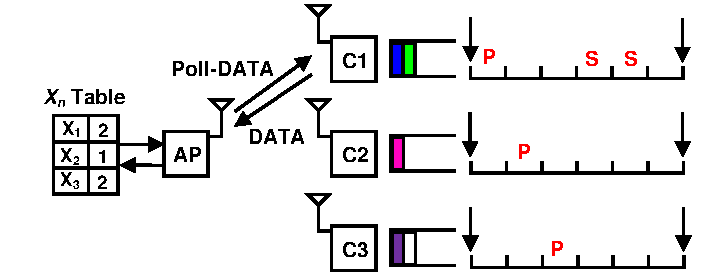
\includegraphics[scale=0.8]{animation_05.pdf}
\end{figure}
\end{frame}

\begin{frame}
\frametitle{Baseline Policy - A Toy Example}
\begin{itemize}
\item Phase 2: AP schedules a client based on Max-Weight policy
\item Max-Weight: select the client that maximizes $p_nX_n$
\end{itemize}
\begin{figure}
\centering
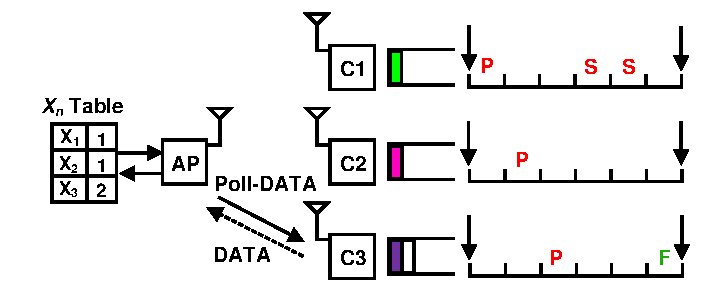
\includegraphics[scale=0.8]{animation_06.pdf}
\end{figure}
\end{frame}



\begin{frame}
\frametitle{Drawbacks of the Baseline Policy}
\begin{itemize}
\item [1] Overhead due to polling
\item [2] Channel utilization for data packets is low
\item [3] Not practical when $N$ is large
\item We propose three solutions to improve polling in phase 1
\end{itemize}
\end{frame}

\section{Proposed Solutions}

\begin{frame}
\frametitle{1. Piggybacked Queue Length}
\begin{itemize}
\item Queue length can be appended in DATA packets
\end{itemize}
\begin{figure}
\centering
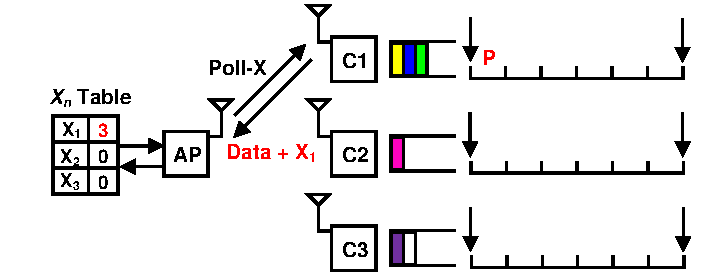
\includegraphics[scale=0.8]{piggyback_1.pdf}
\end{figure}
\end{frame}

\begin{frame}
\frametitle{NS-2 Implementation: Piggybacking}
\end{frame}

\begin{frame}
\frametitle{2. Retry Limit for Polling}
\begin{itemize}
\item Retry limit: avoid polling a client with poor channel indefinitely
\item Example: $p_1=0.1$ and retry limit = 1
\end{itemize}
\begin{figure}
\centering
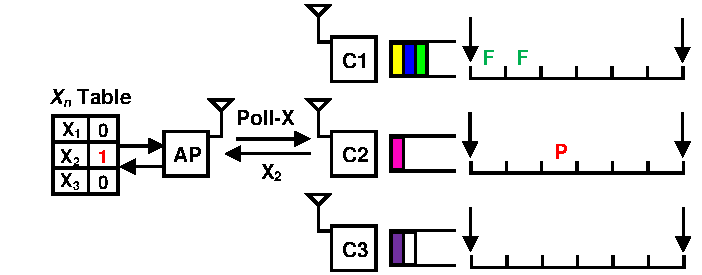
\includegraphics[scale=0.8]{retry_1.pdf}
\end{figure}
\end{frame}

\begin{frame}
\frametitle{NS-2 Implementation: Retry Limit}
\end{frame}

\begin{frame}
\frametitle{3. Selective Polling}
\begin{itemize}
\item Polling a subset of clients: avoid spending too much time on Phase 1 when the network size is large
\item Example: Randomly select 2 out of 3 clients (say C2, C3)
\end{itemize}
\begin{figure}
\centering
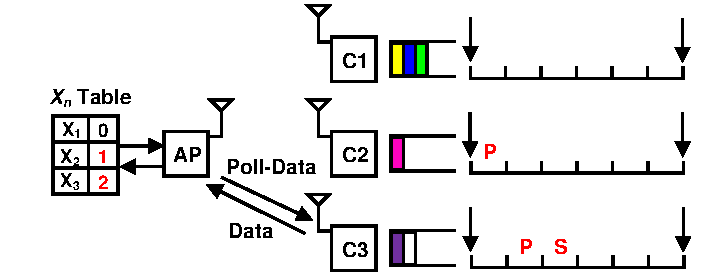
\includegraphics[scale=0.8]{selective_1.pdf}
\end{figure}
\end{frame}

\begin{frame}
\frametitle{NS-2 Implementation: Selection}
\end{frame}

\section{Simulation}
\begin{frame}
\frametitle{Simulation Results}
\end{frame}
\end{document}
